\documentclass{article}
\usepackage{graphicx}
\usepackage{subcaption}
\usepackage{listings}
\usepackage{color}
\usepackage{hyperref}
\usepackage{amsmath}

\renewcommand\lstlistingname{Quelltext} % Change language of section name

\lstset{ % General setup for the package
	language=Perl,
	basicstyle=\small\sffamily,
	numbers=left,
 	numberstyle=\tiny,
	frame=tb,
	tabsize=4,
	columns=fixed,
	showstringspaces=false,
	showtabs=false,
	keepspaces,
	commentstyle=\color{red},
	keywordstyle=\color{blue}
}
\pagenumbering{arabic}
\begin{document}

\begin{titlepage}
	\centering
	
\includegraphics[width=0.4\textwidth]{irif_horizontal}
	
\includegraphics[width=0.4\textwidth]{Logo80ANS_OR}\par\vspace{1cm}
	
\includegraphics[width=0.4\textwidth]{logop7}
	
\includegraphics[width=0.4\textwidth]{Universite_Paris_logo_horizontal}\par\vspace{1cm}
	{\scshape\LARGE Université Paris Diderot \par}
	{\scshape\Large -\par}

	{\scshape\LARGE IRIF \par}
	\vspace{1cm}
	{\scshape\Large Rapport de Stage\par}
	{\scshape\Large du 01/06/2019 au 01/08/2019\par}
	\vspace{1.5cm}
	{\scshape\Large éffectué à Paris\par}
	\vspace{1.5cm}
	{\Large\itshape Sébastien Lecleire\par}
	{\Large\itshape Etudiant en MASTER 1 IMPAIRS\par}
	\vfill
	supervisé par\par
	Mr Yann \textsc{Régis-Gianas}

	\vfill
\end{titlepage}


\newpage

\tableofcontents
\newpage

\section{Remerciements}
Avant tout développement sur cette expérience professionnelle, il apparaît opportun de commencer ce rapport de stage par des remerciements, à ceux qui m’ont beaucoup appris au cours de ce stage, et même à ceux qui ont eu la gentillesse de faire de ce stage un moment très profitable.
\newline
Tout d'abord, j'adresse mes remerciements à ma professeure et amie, Mme Ines Klimann, maître de conférences à l'Université Paris Diderot (Paris 7) qui m'a beaucoup aidé dans ma recherche de stage.
\newline
Je tiens à remercier vivement mon maitre de stage, Mr Yann Régis-Gianas, maître de conférences à l'Université Paris Diderot (Paris 7) et responsable de la platforme LearnOCaml au sein de l'IRIF pour son accueil, son enthousiasme et ses conseils avisés. Grâce à sa confiance j'ai pu accomplir mes différentes missions en totale autonomie avec rigueur et efficacité. Il fut d'une aide précieuse dans les moments les plus délicats.
\newline 
Je remercie également l'ensemble des employés de l'IRIF et de l'Université Paris Diderot (Paris 7) pour leur accueil, leur gentillesse et leur professionnalisme.
Enfin, je tiens à remercier toutes les personnes qui m'ont conseillé et aidé lors de mon stage.


\newpage

\section{Introduction}

Du 01/06/2019 au 01/09/2019, j’ai effectué un stage au sein de l'Institut de Recherche en Informatique Fondamentale (IRIF\footnote{\label{IRIF} Institut de Recherche en Informatique Fondamentale}). Au cours de ce stage dans l'équipe \begin{math}\pi r^2\end{math}, j’ai pu m’intéresser au développement des méthodes formelles ou mathématiques pour modéliser des systèmes existants, naturels ou artificiels, et pour résoudre des problèmes concrets.
Plus largement, ce stage a été l’opportunité pour moi d’appréhender l'aspect pratique de tous les metiers liés au développement d'une application de sa conception à sa mise en production et des méthodes pour rendre plus sûre et plus efficace la distribution de systèmes logiciels de grande dimension.
\newline\newline
Au-delà d’enrichir mes connaissances informatiques, ce stage m’a permis de comprendre énormement de chose sur le travail en équipe, sur les subtilités de la vie en entreprise et m'a donné de nombreuses pistes sur mon orientation après mon Master 2.
Mon stage au pôle Preuves, Programmes et Systèmes (PPS\footnote{\label{PPS} Preuves, Programmes et Systèmes}) de l'IRIF\ref{IRIF} a consisté essentiellement en l'amélioration de la platforme LearnOCaml et au développement d'applications permettant de faciliter et de simplifier son utilisation.
Mon maître de stage étant maître de conférences à l'Université Paris Diderot (Paris 7) et membre permanant du pôle PPS\ref{PPS}, j’ai pu apprendre dans d’excellentes conditions à utiliser de nombreux outils mis à disposition par Github et à réaliser un FrontEnd, un BackEnd, une API\footnote{\label{API} Interface de Programmation d’Application ou Interface de Programmation Applicative}, à administrer des serveurs Cloud Openstack et des Nodes Kubernetes aussi bien en local qu'avec OVH.
\newline\newline
Ce stage a donc été une opportunité pour moi de percevoir comment les recherches menées à l'IRIF\ref{IRIF} reposent sur l’étude et la compréhension des fondements de toute l’informatique, afin d’apporter des solutions innovantes aux défis actuels et futurs des sciences numériques.
L’élaboration de ce rapport a pour principale source les différents enseignements tirés de la pratique journalière des tâches auxquelles j’étais affecté.
\newline\newline
En vue de rendre compte de manière fidèle et analytique des 2 mois passés au sein de l'IRIF\ref{IRIF}, il apparaît logique de présenter à titre préalable le cadre du stage : l'IRIF\ref{IRIF}, et l’environnement du stage, à savoir le secteur PPS\ref{PPS}. Ensuite, il sera précisé les différentes missions et tâches que j’ai pu effectuer au sein du pôle PPS\ref{PPS}. Enfin les nombreux apports que j’ai pu en tirer.

\newpage

\section{L'IRIF}

L'Institut de Recherche en Informatique Fondamentale (IRIF) est une unité mixte de recherche (UMR 8243) entre le CNRS et l'université Paris Diderot, qui héberge deux équipes-projets INRIA. Il est issu de la fusion des deux UMR LIAFA et PPS au 1er janvier 2016. L'IRIF est aussi membre de la Fondation Sciences Mathématiques de Paris (FSMP). 

\subsection{Présentation}

l’IRIF est reconnu pour ses contributions portant sur la conception et l’analyse d’algorithmes, l’étude des modèles de calculs et de représentation des données, les fondements des langages de programmation, le développement logiciel, la vérification et la certification. L’IRIF effectue aussi une recherche interdisciplinaire mettant à profit sa démarche scientifique.
\newline\newline
L’IRIF s'appuie sur des concepts mathématiques développés et étudiés en son sein, notamment en combinatoire, théorie des graphes, logique et algèbre. Ces travaux contribuent aussi directement aux mathématiques, notamment en physique combinatoire, probabilités, catégories, théorie de la preuve, et preuves assistées par ordinateur.
\newline\newline
Au CNRS, l'IRIF est principalement rattaché à l'Institut National des Sciences de l'Information et de leurs Interactions (INS2I) et, secondairement, à l'Institut National des Sciences Mathématiques et de leurs Interactions (INSMI). L'IRIF est membre de l'UFR d'informatique de l'université Paris Diderot, et accueille également en son sein plusieurs membres de l'UFR de mathématiques. Enfin, l'IRIF est associé à l'école doctorale des Sciences Mathématiques de Paris Centre (ED 386).
\newline\newline
L'IRIF est structuré en neuf équipes thématiques regroupées en trois pôles de recherche :
	\begin{itemize}
		\item[$\ast$]Pôle Algorithmes et structures discrètes
		\item[$\ast$]Pôle Automates, structures et vérification
		\item[$\ast$]Pôle Preuves, programmes et systèmes
	\end{itemize}
L'IRIF compte actuellement une centaine de membres permanents, se répartissant environ en 48 enseignants-chercheurs, 27 chercheurs CNRS, 5 chercheurs INRIA, 8 membres émerites et 7 personnels administratifs ou techniques (en janvier 2019). L'effectif total de l'IRIF, incluant doctorants, postdoctorants, et visiteurs de longue durée s'élève à près de deux cents personnes.
\newline\newline
Six membres de l'IRIF ont été lauréats de l'European Research Council (ERC), trois sont membres de l'Institut Universitaire de France (IUF) et deux sont membres de l'Academia Europæa. 

\subsection{PPS}

Thèmes de recherche
\newline\newline
Le programme scientifique du pôle Preuves, programmes et systèmes (PPS) de l'IRIF vise à renforcer les fondements théoriques des langages de programmation, des assistants de preuves et, plus généralement, des formalismes de calcul. Ces problématiques sont abordées en croisant trois points de vue complémentaires :
\begin{itemize}	
	\item[$\ast$]une approche syntaxique, qui développe des langages théoriques issus de formalismes logiques
    \item[$\ast$]une approche algébrique, qui étudie les structures mathématiques liées au calcul
	\item[$\ast$]une approche pratique, qui modélise et analyse des systèmes de calcul réels
\end{itemize}
Le pôle est constitué de trois équipes thématiques, correspondant à chacun de ces trois points de vue. Elles développent leurs outils propres, et les mettent ensuite au service d'objectifs scientifiques communs :
\begin{figure}[h!]
	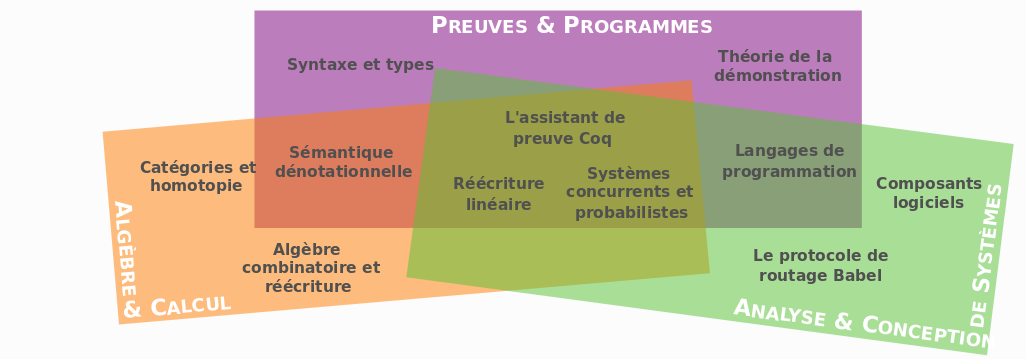
\includegraphics[width=\linewidth]{PPS.png}
	\caption{Diagramme des équipes PPS.}
\end{figure}
\newline
Le pôle PPS héberge l'équipe-projet \begin{math}\pi r^2\end{math} commune à l'INRIA, au CNRS et à l'Université Paris-Diderot — Paris 7, ainsi qu'une partie des membres de l'IRILL (Initiative de Recherche et d'Innovation sur le Logiciel Libre), une structure commune à l'INRIA, à l'Université Paris-Diderot — Paris 7 et à l'Université Pierre-et-Marie-Curie — Paris 6. 
\newpage
\section{Mes missions}

Au cours de ce stage, j’ai eu l’opportunité de découvrir un ensemble de métier sous de nombreuses formes et de comprendre de manière globale les difficultés que les informaticiens pouvaient rencontrer. Pour une meilleure compréhension des tâches que j’ai pu effectuer, il apparaît approprié de traiter en premier lieu des outils qui étaient mis à ma disposition, puis de traiter de manière détaillée les tâches que j’ai pu effectuer.

\subsection{Les outils à ma disposition}

Au cours de ce stage, j’ai passé le plus clair de mon temps à réfléchir et à coder. A mesure que j’apprenais, mes recherches se sont approfondies. Ce n’est donc qu’à partir de la 2e semaine de mon stage que j’ai été véritablement opérationnel, du fait de ma meilleure maîtrise des ressources mises à ma disposition.

\subsubsection{Mon matériel informatique}

A été mis à ma disposition un Dell OptiPlex 7450 All-in-One doté d'un processeur Intel Core i5-7600, d'un SSD de 256GB, de 16GB de RAM et d'un écran 4K. Un vrai bijou de technologie suffisamment puissant pour faire tourner tous les serveurs et toutes les machines virtuelles dont j'avais besoin.
Le tout relié à la fibre de l'université Paris Diderot (Paris 7), j'avais là de quoi travailler sans craindre le moindre problème de performance.

\subsubsection{Ma distribution}

\begin{figure}[h!]
	\centering
  	\begin{subfigure}[b]{0.2\linewidth}
    
\includegraphics[width=\linewidth]{Parrot.png}
  	\end{subfigure}
\end{figure}

Rien de tel qu'une distribution Linux pour travailler ! Et Parrot OS, distribution basée sur Debian mettant l'accent sur la sécurité fut mon choix. Open source et basé sur un OS de la famille POSIX, Parrot OS est une distribution complète et très récente (lancée en 2013) alliant sécurité, modernité et efficacité.
\newpage
\subsubsection{Github}
\begin{figure}[h!]
	\centering
  	\begin{subfigure}[b]{0.4\linewidth}
    
\includegraphics[width=\linewidth]{github.png}
	\end{subfigure}
    \begin{subfigure}[b]{0.5\linewidth}
	
\includegraphics[width=\linewidth]{githubc.jpeg}
	\end{subfigure}
\end{figure}
 
GitHub (exploité sous le nom de GitHub, Inc.) est un service web d'hébergement et de gestion de développement de logiciels, utilisant le logiciel de gestion de versions Git. Ce site est développé en Ruby on Rails et Erlang par Chris Wanstrath, PJ Hyett et Tom Preston-Werner. GitHub propose des comptes professionnels payants, ainsi que des comptes gratuits pour les projets de logiciels libres. Le site assure également un contrôle d'accès et des fonctionnalités destinées à la collaboration comme le suivi des bugs, les demandes de fonctionnalités, la gestion de tâches et un wiki pour chaque projet. 
\newline
Github fonctionne avec le logiciel de contrôle de version Git ce qui signifie qu’il gère les modifications d’un projet sans écraser n’importe quelle partie du projet. Lié de très près au noyaux Linux, Git est installé par défaut sur toutes les distributions Linux et ne risque pas de disparaître de sîtot.

\begin{figure}[h!]
	\centering
  	\begin{subfigure}[b]{0.68\linewidth}
	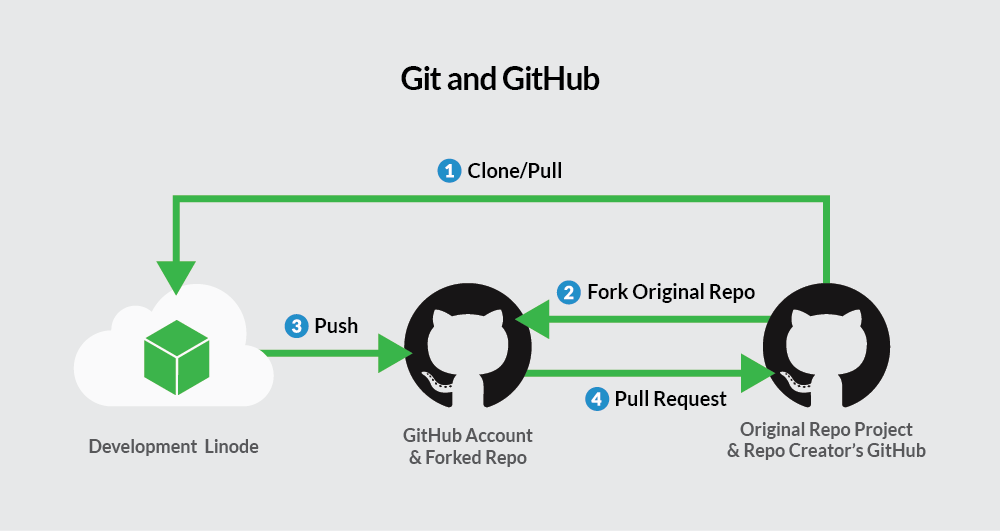
\includegraphics[width=\linewidth]{githubf.png}
	\caption{Fonctionnement en temps normal}	
  	\end{subfigure}
	\begin{subfigure}[b]{0.3\linewidth}
	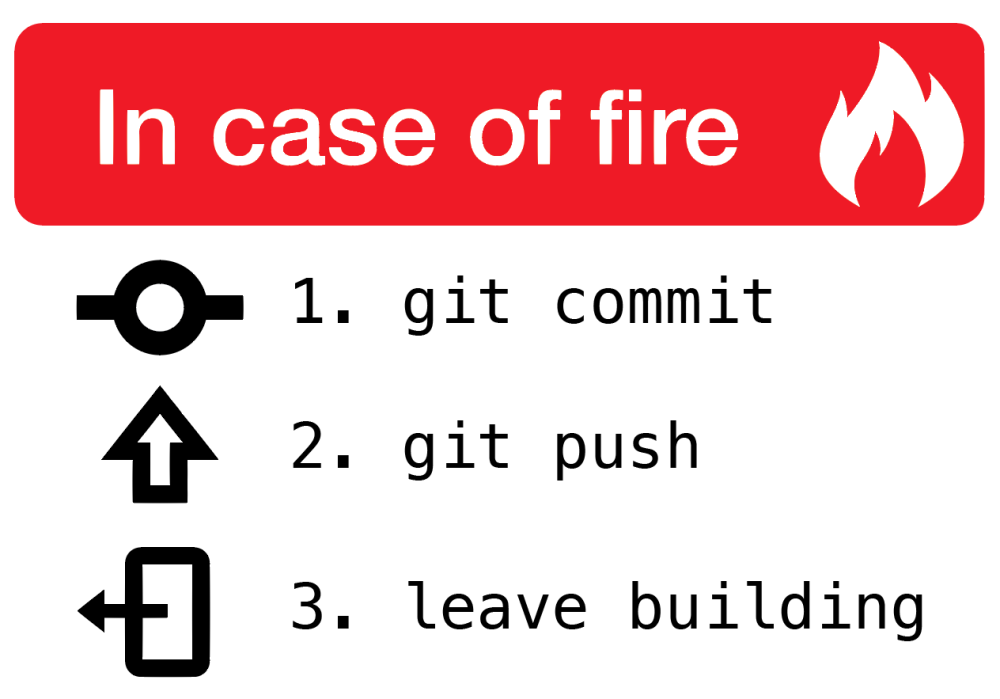
\includegraphics[width=\linewidth]{gitf.png}
	\caption{Fonctionnement en cas de crise majeure}
  \end{subfigure}
\end{figure}

\newpage
\subsubsection{Visual Studio Code}

\begin{figure}[h!]
	\centering
  	\begin{subfigure}[b]{0.1\linewidth}
    
\includegraphics[width=\linewidth]{studio.png}
  	\end{subfigure}
\end{figure}

Visual Studio Code est un éditeur de code extensible, open source et gratuit, développé par Microsoft pour Windows, Linux et macOS. Doté de nombreux plugins, il est parfaitement approprié au développement dans plusieurs langages.

\subsubsection{NodeJS}

\begin{figure}[h!]
	\centering
  	\begin{subfigure}[b]{0.2\linewidth}
    
\includegraphics[width=\linewidth]{Node.png}
  	\end{subfigure}
\end{figure}

Node.js est une plateforme logicielle libre et événementielle en JavaScript orientée vers les applications réseau qui doivent pouvoir monter en charge. 
Elle utilise la machine virtuelle V8 et implémente sous licence MIT les spécifications CommonJS.
Parmi les modules natifs de Node.js, on retrouve http qui permet le développement de serveur HTTP. Il est donc possible de se passer de serveurs web tels que Nginx ou Apache lors du déploiement de sites et d'applications web développés avec Node.js.
Concrètement, Node.js est un environnement bas niveau permettant l’exécution de JavaScript côté serveur.
Node.js est utilisé notamment comme plateforme de serveur Web, elle est utilisée par Groupon, Vivaldi, SAP, LinkedIn, Microsoft, Yahoo!, Walmart, Rakuten, Sage et PayPal.


\subsubsection{npm}

\begin{figure}[h!]
	\centering
  	\begin{subfigure}[b]{0.2\linewidth}
    
\includegraphics[width=\linewidth]{npm.png}
  	\end{subfigure}
\end{figure}

npm est le gestionnaire de paquets officiel de Node.js. npm fonctionne avec un terminal et gère les dépendances pour une application. Il permet également d'installer des applications Node.js disponibles sur le dépôt npm. 
\newpage
\subsubsection{Yarn}

\begin{figure}[h!]
	\centering
  	\begin{subfigure}[b]{0.2\linewidth}
    
\includegraphics[width=\linewidth]{yarn.png}
  	\end{subfigure}
\end{figure}

Yarn est un gestionnaire de dépendances rapide, fiable et sécurisé. C'est un paquet (librairie javascript open source) pour Node.js, un environnement d'éxecution JavaScript permettant d'utiliser ce dernier pour créer des applications webs plus puissantes et maléables notamment grâce à son écosysytème de paquets qui permet de réutiliser du code fait par d'autres développeurs.
Yarn est nous vient des équipes d'ingénieurs de Facebook avec la participation de Google, Exponent et Tilde. C'est une alternative très intéressante à npm qui se veut plus rapide et plus sécurisée !


\subsubsection{Express}

\begin{figure}[h!]
	\centering
  	\begin{subfigure}[b]{0.4\linewidth}
    
\includegraphics[width=\linewidth]{Express.jpeg}
  	\end{subfigure}
\end{figure}

Express est une infrastructure d'applications Web Node.js minimaliste et flexible qui fournit un ensemble de fonctionnalités robuste pour les applications Web et mobiles.
Grâce à une foule de méthodes utilitaires HTTP et de middleware, la création d'une API robuste est simple et rapide. 
\newpage
\subsubsection{Angular}

\begin{figure}[h!]
	\centering
  	\begin{subfigure}[b]{0.4\linewidth}
    
\includegraphics[width=\linewidth]{Angular.jpeg}
  	\end{subfigure}
\end{figure}

Angular (communément appelé "Angular 2+" ou "Angular v2 et plus") est un framework côté client open source basé sur TypeScript dirigée par l'équipe du projet Angular à Google et par une communauté de particuliers et de sociétés. Angular est une réécriture complète de AngularJS, cadriciel construit par la même équipe. 

\begin{figure}[h!]
	\centering
	\begin{subfigure}[b]{0.9\linewidth}
  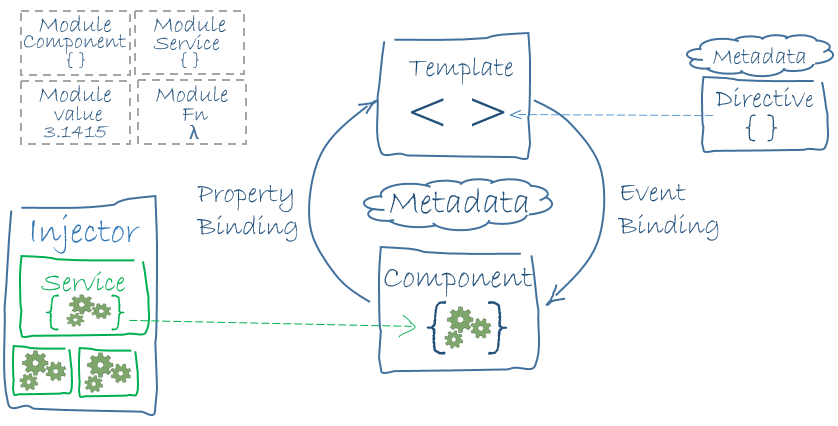
\includegraphics[width=\linewidth]{Angularf.png}
	\end{subfigure}
	\caption{L'Architecture de l'application. Les principaux blocs de construction sont des modules, des composants, des modèles, des métadonnées, la liaison de données, des directives, des services et de l'injection de dépendance.}
\end{figure}
\newpage
\subsubsection{Kubernetes}

\begin{figure}[h!]
	\centering
  	\begin{subfigure}[b]{0.4\linewidth}
    
\includegraphics[width=\linewidth]{kube.png}
  	\end{subfigure}
\end{figure}

Kubernetes (communément appelé "K8s") est un système open source qui vise à fournir une plate-forme permettant d'automatiser le déploiement, la montée en charge et la mise en œuvre de conteneurs d'application sur des clusters de serveurs. Il fonctionne avec toute une série de technologies de conteneurisation, et est souvent utilisé avec Docker. Il a été conçu à l'origine par Google, puis offert à la Cloud Native Computing Foundation. 
\newline
\begin{figure}[h!]
	\centering
  	\begin{subfigure}[b]{1.0\linewidth}
	\includegraphics[width=\linewidth]{kubernetes.png}
	\caption{Plan de contrôle Kubernetes}
  	\end{subfigure}
\end{figure}

Le maître Kubernetes est l'unité de contrôle principale qui gère la charge de travail et dirige les communications dans le système. Le plan de contrôle de Kubernetes consiste en plusieurs composants, chacun ayant son propre processus, qui peuvent s'exécuter sur un seul node maître ou sur plusieurs maîtres permettant de créer des clusters haute disponibilité. Les différents composants du plan de contrôle de Kubernetes sont décrits à la page suivante.
\newpage
\textbf{Les différents composants du plan de contrôle de Kubernetes : }
\newline
\newline
\textbf{etcd}
\newline
\newline
etcd est une unité de stockage distribuée persistante et légère de données clé-valeur développée par CoreOS, qui permet de stocker de manière fiable les données de configuration du cluster, représentant l'état du cluster à n'importe quel instant. D'autres composants scrutent les changements dans ce stockage pour aller eux-mêmes vers l'état désiré.
\newline
\newline
\textbf{serveur d'API}
\newline
\newline
Le serveur d'API est un élément clé et sert l'API Kubernetes grâce à JSON via HTTP. Il fournit l'interface interne et externe de Kubernetes. Le serveur d'API gère et valide des requêtes REST et met à jour l'état des objets de l'API dans etcd, permettant ainsi aux clients de configurer la charge de travail et les containers sur les nœuds de travail.
\newline
\newline
\textbf{L'ordonnanceur}
\newline
\newline
L'ordonnanceur est un composant additionnel permettant de sélectionner quel node devrait faire tourner un pod non ordonnancé en se basant sur la disponibilité des ressources. L'ordonnanceur gère l'utilisation des ressources sur chaque node afin de s'assurer que la charge de travail n'est pas en excès par rapport aux ressources disponibles. Pour accomplir cet objectif, l'ordonnanceur doit connaître les ressources disponibles et celles actuellement assignées sur les serveurs.
\newline
\newline
\textbf{Controller manager}
\newline
\newline
Le gestionnaire de contrôle (controller manager) est le processus dans lequel s'exécutent les contrôleurs principaux de Kubernetes tels que DaemonSet Controller et le Replication Controller. Les contrôleurs communiquent avec le serveur d'API pour créer, mettre à jour et effacer les ressources qu'ils gèrent (pods, service endpoints, etc.).
\newline
\newline
\textbf{Node Kubernetes}
\newline
\newline
Le Node aussi appelé Worker ou Minion est une machine unique (ou une machine virtuelle) où des conteneurs (charges de travail) sont déployés. Chaque node du cluster doit exécuter le programme de conteneurisation (par exemple Docker), ainsi que les composants mentionnés ci-dessous, pour communiquer avec le maître afin de configurer la partie réseau de ces conteneurs.
\newline
\newline
\newline
\newline
\textbf{Kubelet}
\newline
\newline
Kubelet est responsable de l'état d'exécution de chaque nœud (c'est-à-dire, d'assurer que tous les conteneurs sur un nœud sont en bonne santé). Il prend en charge le démarrage, l'arrêt, et la maintenance des conteneurs d'applications (organisés en pods) dirigé par le plan de contrôle.
\newline
\newline
Kubelet surveille l'état d'un pod et s'il n'est pas dans l'état voulu, le pod sera redéployé sur le même node. Le statut du node est relayé à intervalle de quelques secondes via messages d’état vers le maître. Dès que le maître détecte un défaut sur un node, le Replication Controller voit ce changement d'état et lance les pods sur d'autres hôtes en bonne santé.
\newline
\newline
\textbf{Kube-proxy}
\newline
\newline
Le kube-proxy est l’implémentation d'un proxy réseau et d'un répartiteur de charge, il gère le service d'abstraction ainsi que d'autres opérations réseaux. Il est responsable d'effectuer le routage du trafic vers le conteneur approprié en se basant sur l'adresse IP et le numéro de port de la requête entrante.
\newline
\newline
\textbf{cAdvisor}
\newline
\newline
cAdvisor est un agent qui surveille et récupère les données de consommation des ressources et des performances comme le processeur, la mémoire, ainsi que l'utilisation disque et réseau des conteneurs de chaque node. 
\newline
\newline
\newpage
\subsubsection{Openstack}

\begin{figure}[h!]
	\centering
  	\begin{subfigure}[b]{0.4\linewidth}
    
\includegraphics[width=\linewidth]{open.png}
  	\end{subfigure}
\end{figure}

OpenStack est un ensemble de logiciels open source permettant de déployer des infrastructures de cloud computing (infrastructure en tant que service). La technologie possède une architecture modulaire composée de plusieurs projets corrélés (Nova, Swift, Glance...) qui permettent de contrôler les différentes ressources des machines virtuelles telles que la puissance de calcul, le stockage ou encore le réseau inhérents au centre de données sollicité.
\newline
Le projet est porté par la Fondation OpenStack, une organisation non-commerciale qui a pour but de promouvoir le projet OpenStack ainsi que de protéger et d'aider les développeurs et toute la communauté OpenStack.
\newline
De nombreuses entreprises ont rejoint la fondation OpenStack. Parmi celles-ci on retrouve : Canonical, Red Hat, SUSE, eNovance, AT\&T, Cisco, Dell, IBM, Yahoo!, Oracle, Orange, Cloudwatt, EMC, VMware, Intel, OVH, NetApp. 

\begin{figure}[h!]
	\centering
  	\begin{subfigure}[b]{0.85\linewidth}
	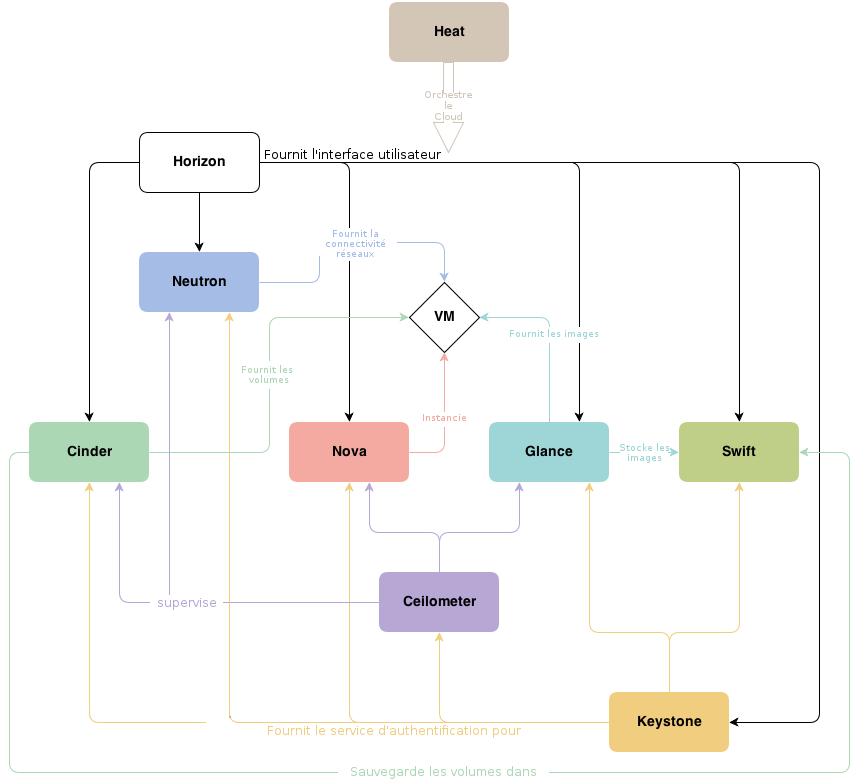
\includegraphics[width=\linewidth]{openstack.png}
	\caption{Architecture conceptuelle des services OppenStack}
  	\end{subfigure}
\end{figure}
\newpage
OpenStack possède une architecture modulaire qui comprend de nombreux composants, nous ne nous intéresserons qu'à deux d'entre eux : \textit{Swift} et \textit{Cinder}
\newline
\newline
\textbf{Stockage objet : Swift}

\begin{figure}[h!]
	\centering
  	\begin{subfigure}[b]{1.0\linewidth}
	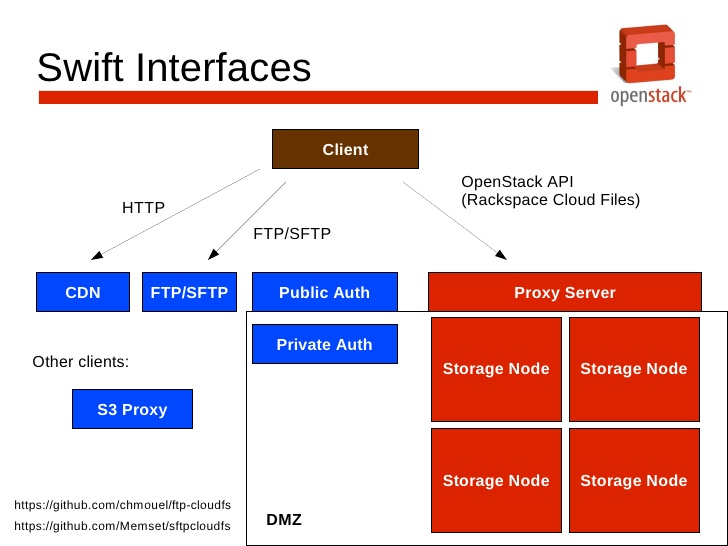
\includegraphics[width=\linewidth]{swift.jpeg}
	\caption{Architecture conceptuelle des services Swift}
  	\end{subfigure}
\end{figure}

Le stockage objet d'OpenStack s'appelle Swift. C'est un système de stockage de données redondant et évolutif. Les fichiers sont écrits sur de multiples disques durs répartis sur plusieurs serveurs dans un Datacenter. Il s'assure de la réplication et de l'intégrité des données au sein du cluster. Le cluster Swift évolue horizontalement en rajoutant simplement de nouveaux serveurs. Si un serveur ou un disque dur tombe en panne, Swift réplique son contenu depuis des nœuds actifs du cluster dans des emplacements nouveaux. Puisque toute la logique de Swift est applicative, elle permet l'utilisation de matériel peu coûteux et non spécialisé.
\newline
En août 2009, c'est Rackspace qui a commencé le développement de Swift, en remplacement de leur ancien produit nommé Cloud Files. Aujourd'hui c'est la société SwiftStack qui mène le développement de Swift avec la communauté.

\newpage
\textbf{Stockage bloc : Cinder}
\newline

\begin{figure}[h!]
	\centering
  	\begin{subfigure}[b]{1.0\linewidth}
	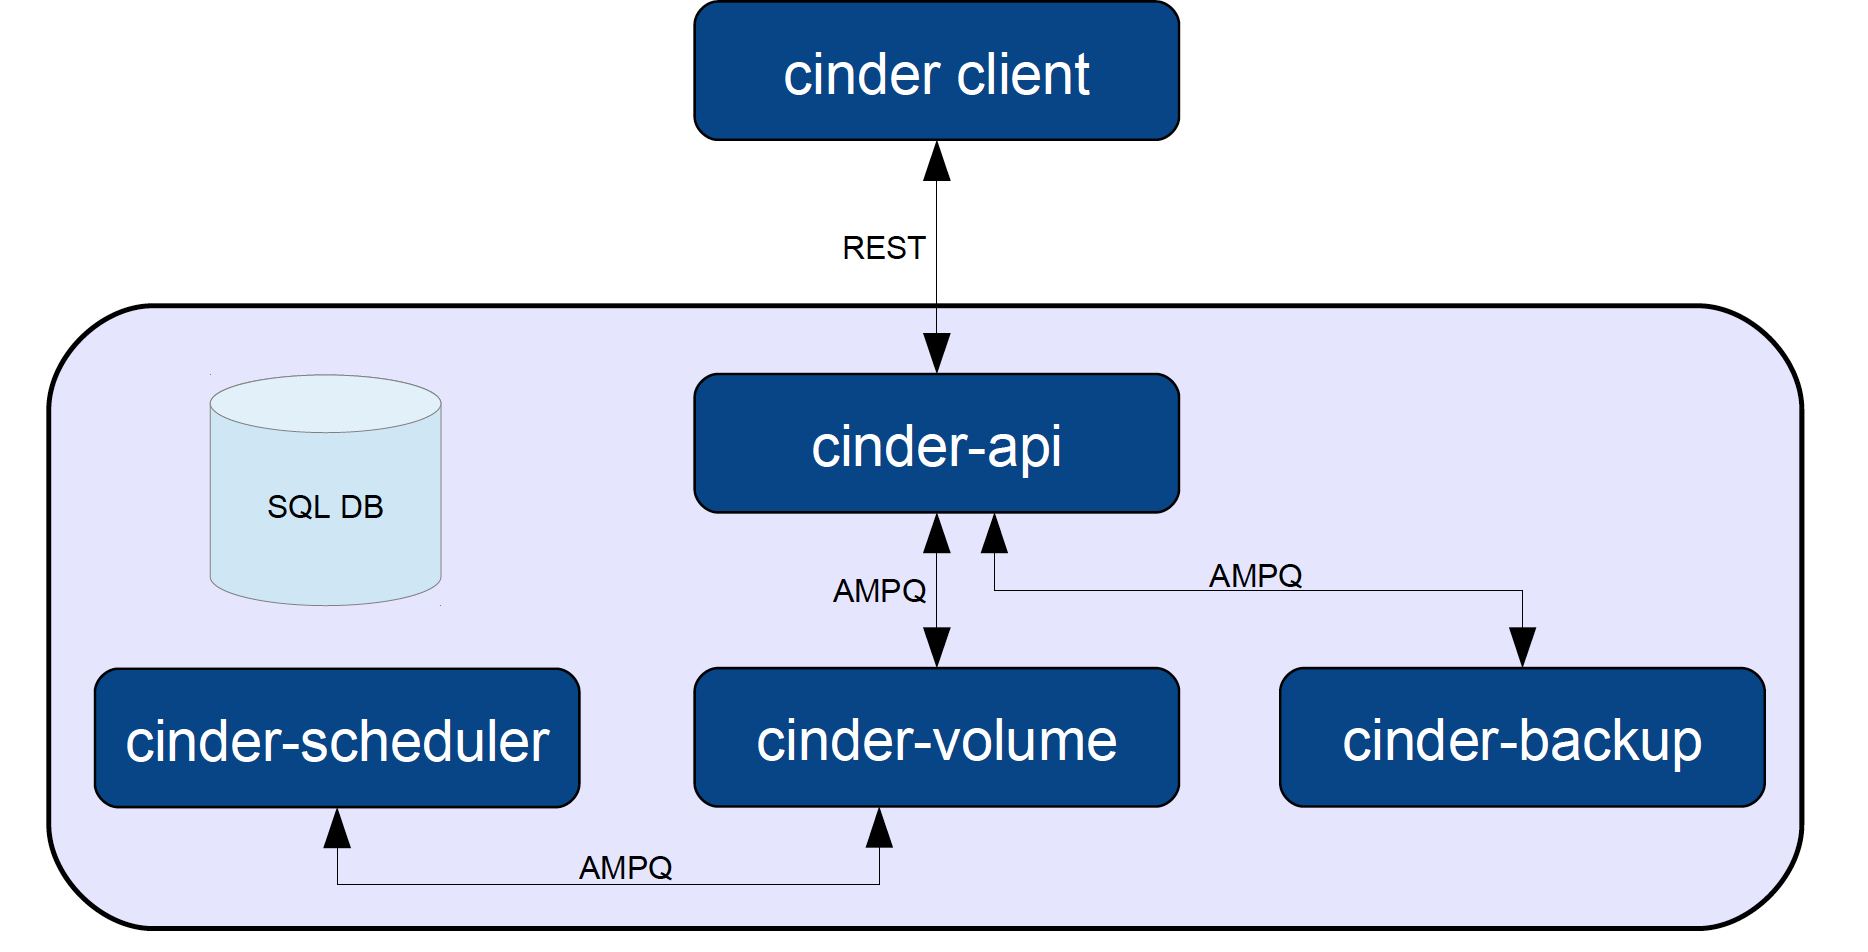
\includegraphics[width=\linewidth]{cinder.png}
	\caption{Architecture conceptuelle des services Cinder}
  	\end{subfigure}
\end{figure}

Le service de stockage en mode bloc d'OpenStack s'appelle Cinder. Il fournit des périphériques persistants de type bloc aux instances OpenStack. Il gère les opérations de création, d'attachement et de détachement de ces périphériques sur les serveurs. En plus du stockage local sur le serveur, Cinder peut utiliser de multiples plateformes de stockage tel que Ceph, EMC (ScaleIO, VMAX et VNX), GlusterFS, Hitachi Data Systems, IBM Storage (Storwize family, SAN Volume Controller, XIV Storage System, et GPFS), NetApp, HP (StoreVirtual et 3PAR) et bien d'autres.
\newline
Le stockage en mode bloc est utilisé pour des scénarios performant comme celui du stockage de base de données, mais aussi pour fournir au serveur un accès bas niveau au périphérique de stockage. Cinder gère aussi la création d'instantanés (snapshots), très utile pour sauvegarder des données contenues dans les périphériques de type bloc. Les instantanés peuvent être restaurés ou utilisés pour créer de nouveaux volumes.
\newpage

\subsubsection{Docker}

\begin{figure}[h!]
	\centering
  	\begin{subfigure}[b]{1.0\linewidth}
	
\includegraphics[width=\linewidth]{docker.png}
  	\end{subfigure}
\end{figure}

Docker est un logiciel libre permettant facilement de lancer des applications dans des conteneurs logiciels.
\newline
Selon la firme de recherche sur l'industrie 451 Research, Docker est un outil qui peut empaqueter une application et ses dépendances dans un conteneur isolé, qui pourra être exécuté sur n'importe quel serveur. Il ne s'agit pas de virtualisation, mais de conteneurisation, une forme plus légère qui s'appuie sur certaines parties de la machine hôte pour son fonctionnement. Cette approche permet d'accroître la flexibilité et la portabilité d’exécution d'une application, laquelle va pouvoir tourner de façon fiable et prédictible sur une grande variété de machines hôtes, que ce soit sur la machine locale, un cloud privé ou public, une machine nue, etc..
\newline
Techniquement, Docker étend le format de conteneur Linux standard, LXC, avec une API de haut niveau fournissant une solution pratique de virtualisation qui exécute les processus de façon isolée. Pour arriver à ses fins, Docker utilise entre autres LXC, cgroups et le noyau Linux lui-même. Contrairement aux machines virtuelles traditionnelles, un conteneur Docker n'inclut pas de système d'exploitation, mais s'appuie au contraire sur les fonctionnalités du système d’exploitation fournies par la machine hôte.

\begin{figure}[h!]
	\centering
  	\begin{subfigure}[b]{0.55\linewidth}
	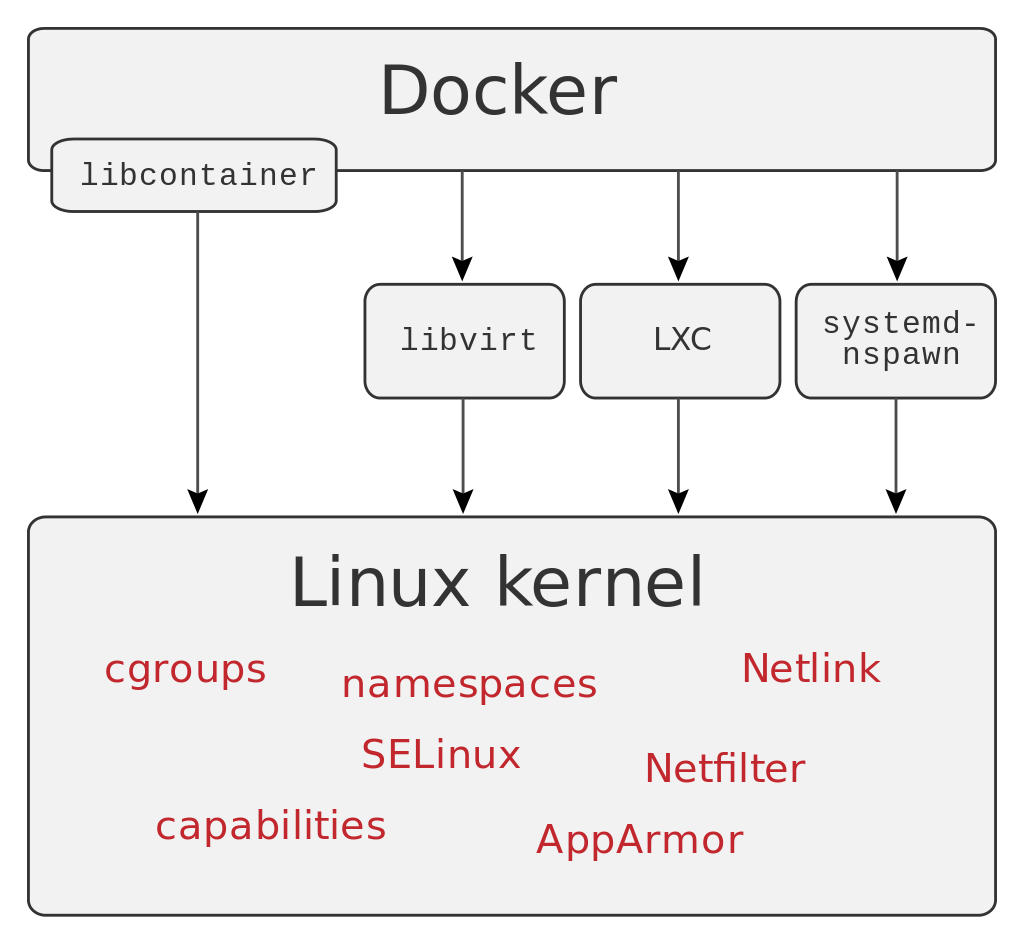
\includegraphics[width=\linewidth]{dockeri.png}
	\caption{Schéma des interfaces de Docker}
  	\end{subfigure}
\end{figure}
\newpage

\subsubsection{Thinkster}
\begin{figure}[h!]
	\centering
  	\begin{subfigure}[b]{0.55\linewidth}
	
\includegraphics[width=\linewidth]{thinkster.png}
  	\end{subfigure}
\end{figure}
\subsubsection{ReadTheDocs}
\subsubsection{LearnOCaml}
\subsubsection{JsOfOCaml}
\subsubsection{Langages utilisés}







\subsection{les missions (responsabilités, tâches à effectuer, dossiers confiés, objectifs)}

\subsection{le bilan
résultats obtenus ( appréciation du maître de stage - productivité ... gestion du temps)
difficultés rencontrées et solutions apportées
enseignements/apports du stage (connaissances - compétences)}

\newpage

\section{Les apports du stage}
Merci !

\subsection{Subsection}

\newpage

\section{Conclusion}

Ce stage a été très enrichissant pour moi car il m’a permis de découvrir dans le détail le secteur du ………, ses acteurs, contraintes… et il m’a permis de participer concrètement à ses enjeux au travers de mes missions variées comme celle du …. que j’ai particulièrement apprécié. Ce stage m’a aussi permis de comprendre que les missions créatives n’étaient pas les plus adaptées pour moi…et je préfère m’orienter vers les métiers de …. qui me conviennent mieux.(Cette partie doit faire le bilan des plus et moins du stage / votre enrichissement pour votre future carrière)


L’entreprise … qui m’a accueilli pendant ce stage fait face à une période charnière…, et je suis très fier d’avoir pu contribuer, participer à cette révolution. L’évolution des usages et l’adaptation de l’entreprise au changement de son environnement….
(Cette partie doit montrer que vous avez su comprendre les enjeux économiques des secteurs de l’entreprise et/ou réponse à la problématique du rapport)


Fort de cette expérience et en réponse à ses enjeux, j’aimerai beaucoup par la suite essayer de m’orienter via un prochain stage, vers le secteur … avec des acteurs de petites tailles, et un important développement d’avenir.
(ouverture …prochaine étape)


\newpage
\section{Tests}
\begin{figure}[h!]
  \centering
  \begin{subfigure}[b]{0.2\linewidth}
    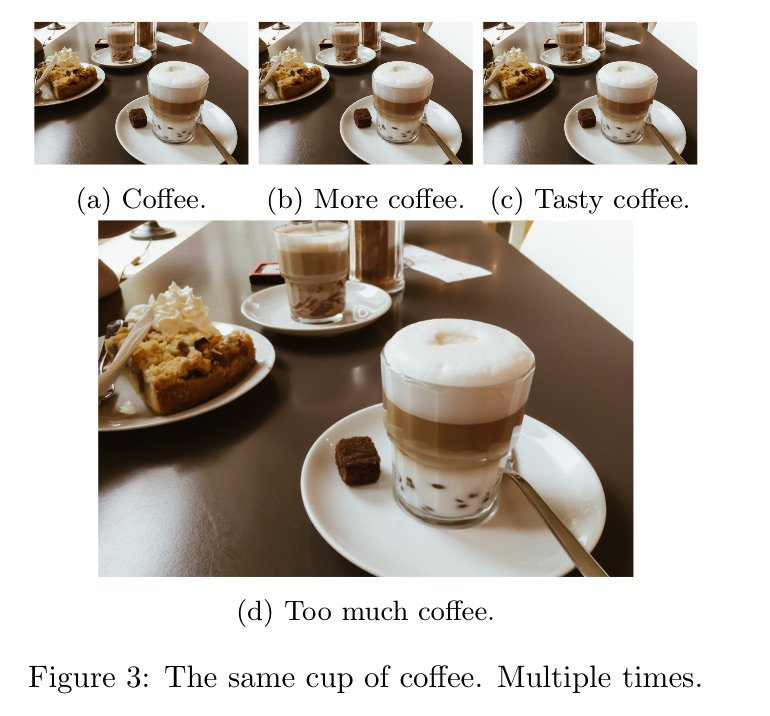
\includegraphics[width=\linewidth]{coffee.jpg}
     \caption{Coffee.}
  \end{subfigure}
  \begin{subfigure}[b]{0.2\linewidth}
    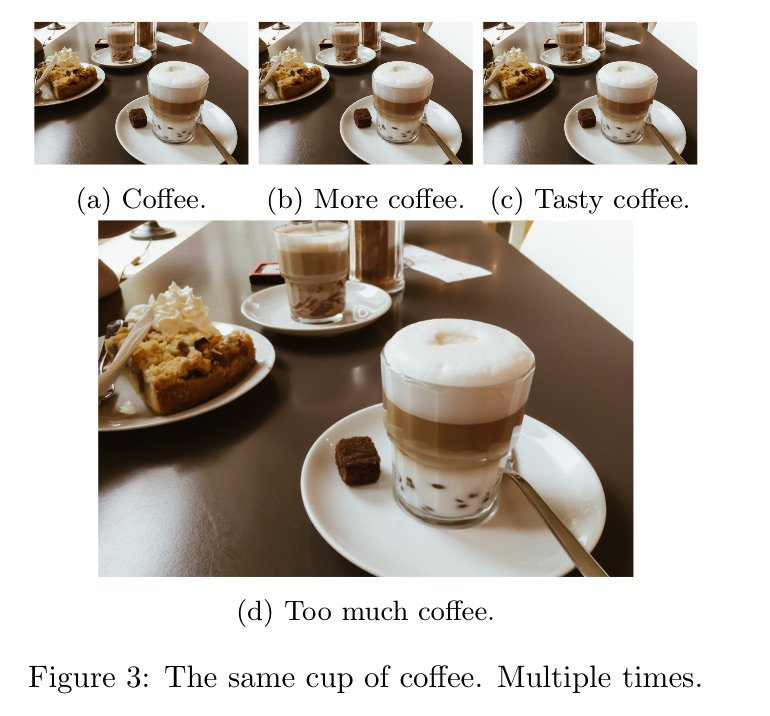
\includegraphics[width=\linewidth]{coffee.jpg}
    \caption{More coffee.}
  \end{subfigure}
  \begin{subfigure}[b]{0.2\linewidth}
    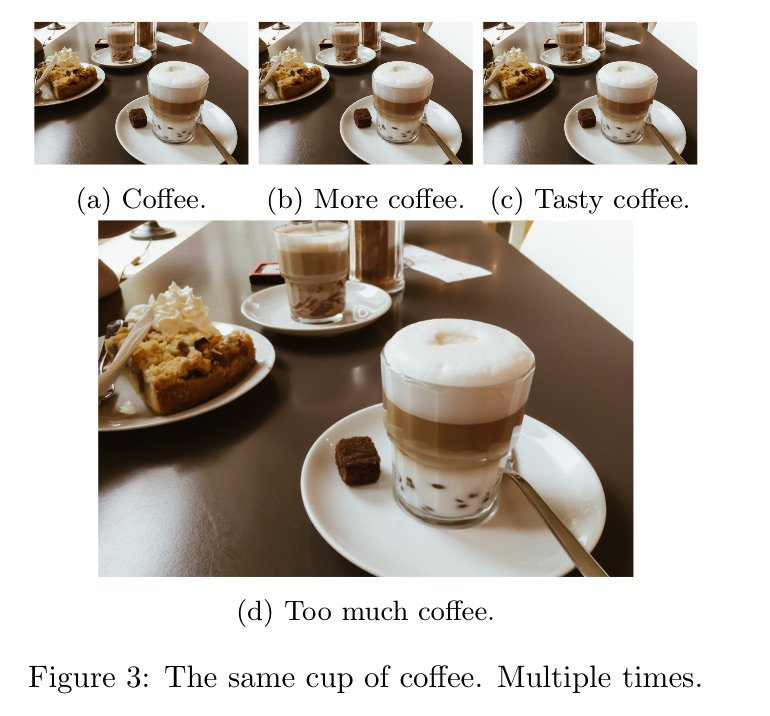
\includegraphics[width=\linewidth]{coffee.jpg}
    \caption{Tasty coffee.}
  \end{subfigure}
  \begin{subfigure}[b]{0.5\linewidth}
    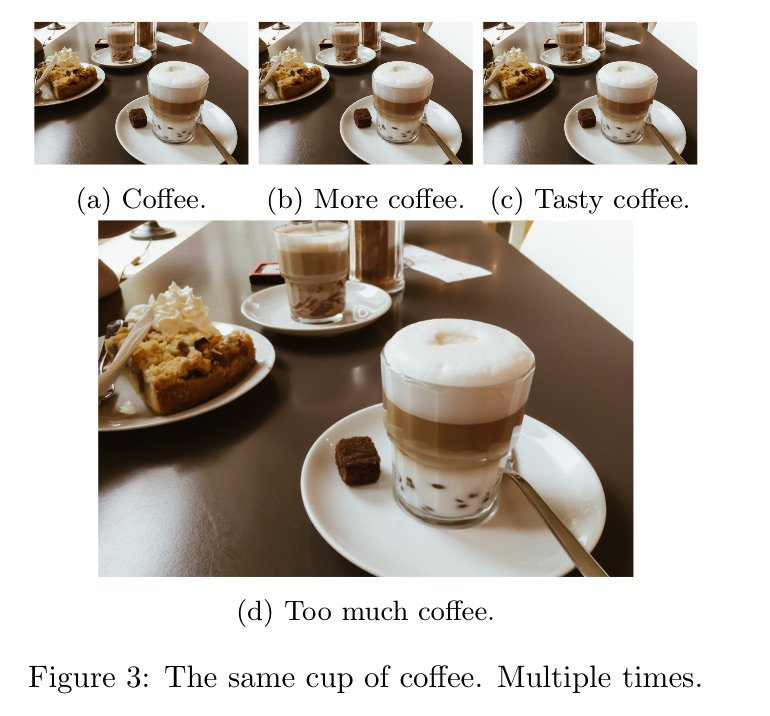
\includegraphics[width=\linewidth]{coffee.jpg}
    \caption{Too much coffee.}
  \end{subfigure}
  \caption{The same cup of coffee. Multiple times.}
  \label{fig:coffee3}
 
\end{figure}

Test of a link : \href{http://www.atec.com}{ici}

Random citation \cite{WEBSITE:1} embeddeed in text.

\begin{lstlisting}
#!/usr/bin/perl
print S(@ARGV);sub S{$r=(@_[0]%4==0&&@_[0]%100!=0)||@_[0]%400=0;}
\end{lstlisting}

\newpage

\bibliography{library}
\bibliographystyle{ieeetr}
http://www.slideshare.net/reidrac/deploying-openstack-object-storage-swift
https://cloudarchitectmusings.com/2013/11/18/laying-cinder-block-volumes-in-openstack-part-1-the-basics/
https://www.aquasec.com/wiki/display/containers/Docker+Architecture
\end{document}
